\chapter{Experiments}\label{sec:experiments}
The experiments are split into two different parts that go in order over the two previous chapters:
\begin{enumerate}
  \item (\cref{sec:exp_weights,sec:exp_cov,sec:exp_acc,sec:exp_conflicts}): Properties of the underlying \markov of \cref{algo:sampler} that are independent of the chosen algorithm.
  \item (\cref{sec:exp_seq,sec:exp_batch,sec:exp_neighbor}): Properties of the proposed algorithms in \cref{sec:uniform_sampling,sec:parallel_sampling}.
\end{enumerate}
We conduct all experiments with the following input parameters and repeat each combination $10$ times.
\begin{itemize}
  \item Random graphs drawn from $\gnp(n,\degavg), \dsf(n,\degavg), \rhg(n,\degavg)$ graphs with $n = 10000$ and $\degavg \in \set{10, 20, 50}$.
  \item Initial weight functions $w \in \set{\wmax, \wunif, \wzero}$.
  \item Number of MCMC-steps $\steps = 10^8$.
  \item Integer weights in $\wInt = [-100,100]$.
\end{itemize}
Due to a very high number of isolated nodes and consequently SCCs in \dsf graphs, we instead extract the largest SCC of the generated \dsf graph and ran all algorithms on its induced subgraph.
To match the number of nodes and edges in this subgraph as best as possible with the intended number of nodes and edges, we modify the initial parameters\footnote{
  All these values were found experimentelly using a binary search by hand. 
} to 
\begin{itemize}
  \item $(n, \degavg) = (25000, 6)$ which led to a SCC with roughly $10000$ nodes and average degree $10$.
  \item $(n, \degavg) = (20000, 14)$ which led to a SCC with roughly $10000$ nodes and average degree $20$.
  \item $(n, \degavg) = (17000, 47)$ which led to a SCC with roughly $10000$ nodes and average degree $50$.
\end{itemize}

We also focus on the following questions for each experiment:

\paragraph{What impact does the underlying graph model have?}
As discussed in \cref{sec:random_graphs}, \rhg and \dsf graphs both are \qq{scale-free} and their degrees follow a power-law distribution whereas edges in \gnp graphs are independent of each other and therefore degrees follow a binomial distribution.
Additionally, \rhg graphs are originally undirected and thus have a reversed edge for every edge in the graph.
Due to this, \rhg graphs have on average the most cycles and the shortest cycles of all three models whereas \dsf graphs are the most acyclic, \ie have the least number of cycles in expectation.

\paragraph{What impact does the average degree have?}
Obviously, graphs of the same random graph class have no significant structural change for bigger average degrees.
But, a bigger average degree translates into a higher number of edges and thus also a higher number of cycles (and possibly shorter cycles) in the graphs.


\paragraph{What impact does the initial weight function have?}
If the average weight is higher, the probability of accepting a proposed weight change consequently also rises.
While there are definitely some scenarios in which a few select number of edges contribute significantly to the high average weight whereas every other edge has a very low weight, these are definitely highly improbable as we assume some kind of uniform distribution in edge-weights across the graph.

\bigskip

\noindent
\textit{%
  All experiments were implemented in \textsc{Rust}\footnote{\url{https://www.rust-lang.org/}} and run on the Goethe-NHR cluster\footnote{\url{https://csc.uni-frankfurt.de/}}.
  We only used nodes with two \texttt{Intel Xeon Skylake Gold 6148} processors with a total of $40$ cores and $192$ GB RAM per node. The implementation can be found on \textsc{GitHub}\footnote{\url{https://github.com/lukasgeis/negative_edge_weights}}.
}


\section{Weight Distributions}\label{sec:exp_weights}
We first study the distribution of edge weights.
Since, for each of the $27$ possible settings ($3$ graph models, $3$ average degrees, $3$ initial weight functions), we have $10^8$ rounds in which we can examine the weight distribution over $201$ possible weights, the sheer amound of data warrants a reduction to a few key aspects.
For this, we first investigate weight distributions as a whole over time in some fixed intervals.

\begin{figure}[!tb]
  \centering
  \makebox[\textwidth][c]{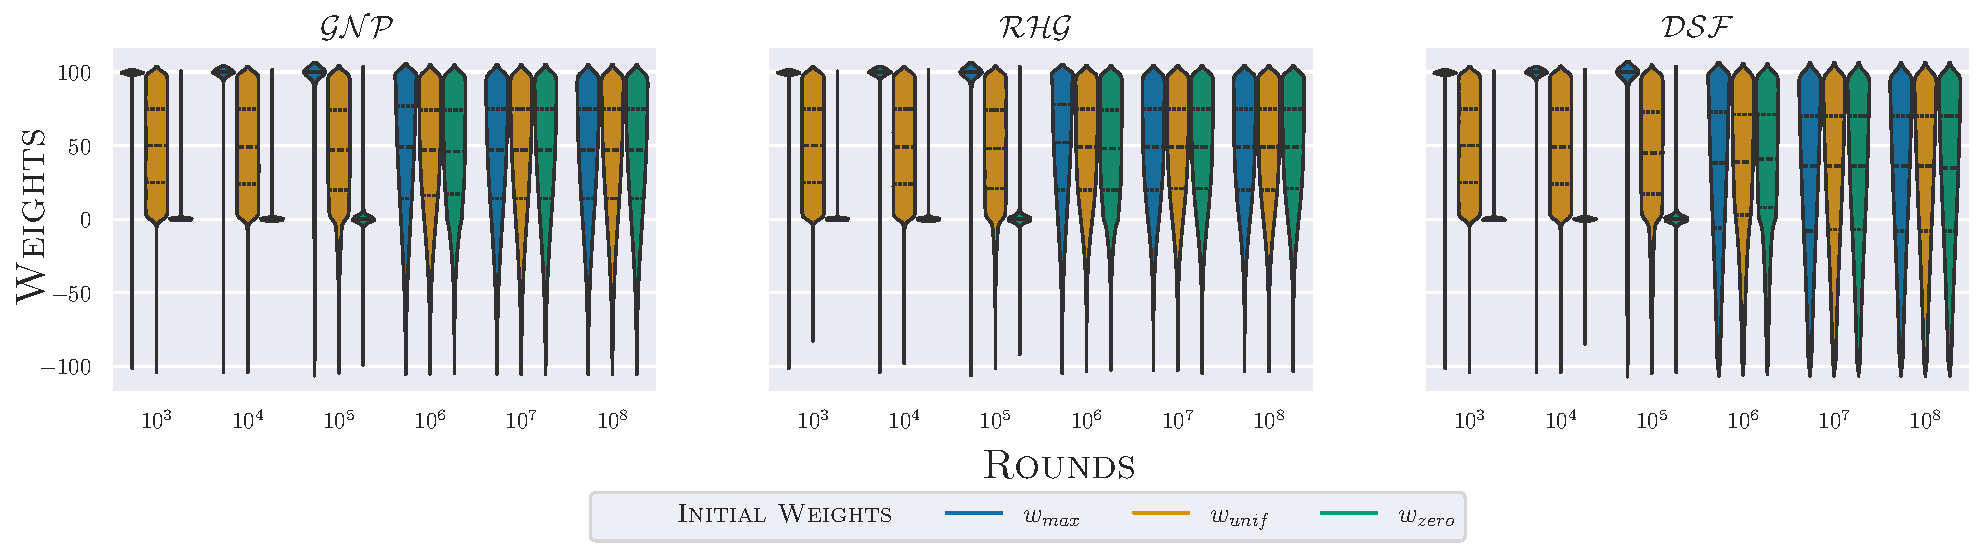
\includegraphics[width=1.2\textwidth]{Figures/experiments/Weights_10.pdf}}
  \caption{
    Weight distributions over time for different graphs with $n = 10000$ nodes and average degree $\degavg = 10$. 
  }
  \label{fig:dist_over_time}
\end{figure}

\begin{figure}[!tb]
  \centering
  \makebox[\textwidth][c]{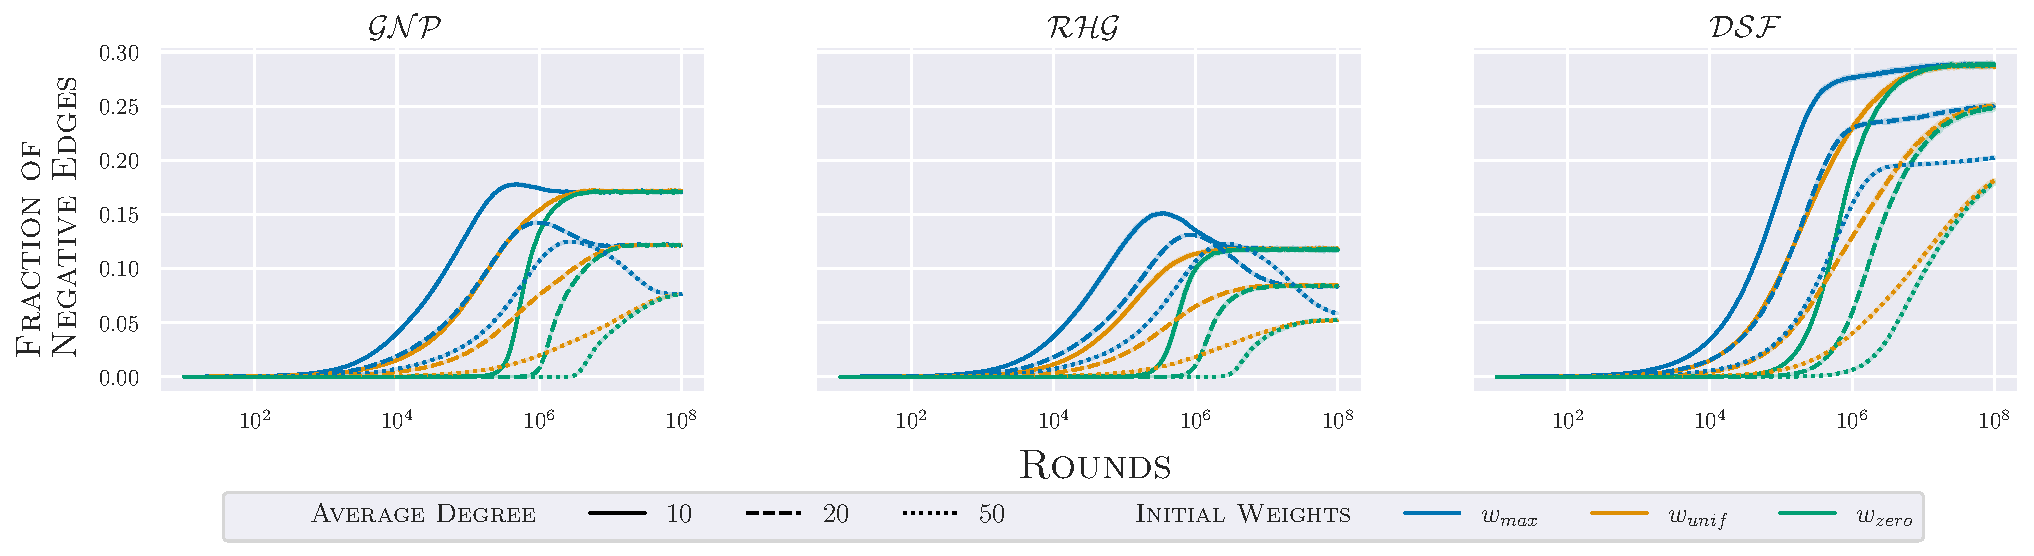
\includegraphics[width=1.2\textwidth]{Figures/experiments/Neg.pdf}}
  \caption{
    Fraction of edges with negative weights over time for different graph models with $n = 10000$ nodes and average degree $\degavg \in \set{10, 20, 50}$.
  }
  \label{fig:neg_edges}
\end{figure}


While weights are uniformly drawn from the symmetric interval $[-100,100]$, since we reject negative cycles, the average weight in strongly connected graphs must always be non-negative\footnote{
  Under the assumption that the graph is strongly connected. 
  Otherwise a single edge not part of any SCC could potentially lower the average weight below $0$.
}.
Because extremely low weights are highly likely to get rejected and extremely high weights are highly likely to be changed in later rounds, we expect distributions to have a peak around some weight and be linearly decreasing in probability mass in both directions.
Also, the impact of the initial weight function should be negligible in higher rounds since all instances converge to the same distributions regardless of starting weights.

\cref{fig:dist_over_time} displays the weight distributions at fixed rounds $10^i$ for $i = 3,\ldots,8$.
The complete dataset can be seen in \cref{fig:app_weight_over_time}.
Clearly, independent of initial weight function, in each instance, all weight distributions converge to a similar one in roughly $10^7$ steps.
This \emph{final} weight distribution is also centered around an average of roughly $50$ with slight variations depending on the chosen graph model and average degree: less cycles lead to lower weights as more weight decreases get accepted whereas more and shorter cycles lead to higher weights as more weight decreases get rejected (see $\dsf(\degavg = 10)$ and $\rhg(\degavg = 50)$ for extremes).


Additionally, while instances that started with $\wmax$ already have extremely low weights after $10^3$ rounds, instances that started with $\wzero$ have almost no negative weight for the first $10^5$ rounds. 
This can be further observed in \cref{fig:neg_edges} which plots the fraction of edges with negative weight over time.
As one would expect, instances of the same model and average degree converge to a fixed fraction independent of the initial weight function.
Also, less cycles lead to higher fractions with $\dsf$ graphs achieving fractions almost twice as high as $\rhg$ graphs.

Surprisingly, for initial weight function $\wmax$, the \markov seems to \qq{overshoot} the fraction of negative edges as at the beginning we have many extremely high edge weights that allow for many (small) negative weights.
As this fraction of extremely high weights gradually decreases over time, the fraction of negative edges concurs and also decreases again until it reaches a stable state.
$\wunif$ instances fall almost directly in the middle between $\wmax$ and $\wzero$ curves which suggests that one could parametrize initial weight functions (possibly by average weight) to interpolate between $\wmax$ and $\wzero$ curves.


\subsection*{Total Variation Distance}
\begin{figure}[!tb]
  \centering
  \makebox[\textwidth][c]{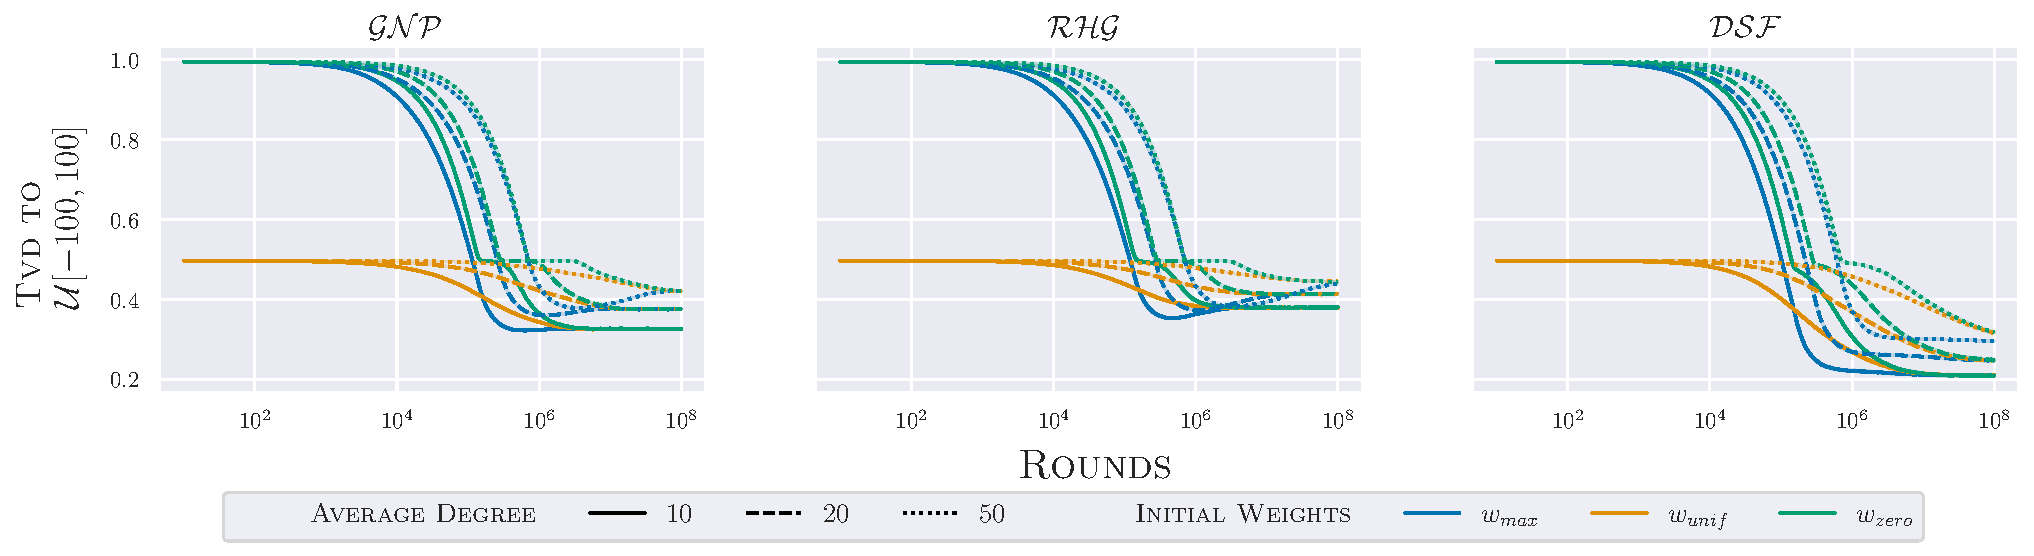
\includegraphics[width=1.2\textwidth]{Figures/experiments/Tvd.pdf}}
  \caption{
    Total variation distance to $\unif[-100,100]$ over time for different graph models with $n = 10000$ nodes and average degree $\degavg \in \set{10, 20, 50}$.
  }
  \label{fig:tvd}
\end{figure}

Another measure for converging distributions is the total variation distance (\textsc{Tvd})\footnote{
  \textsc{Tvd} was implicitly defined in \cref{def:mixing_time} as the term that should be less than $\epsilon$.
} to the distribution in the limit $\pi$.
But since we established in \cref{sec:hardness} that the limit distribution is very hard to compute as it requires some form of enumeration of all feasible states (and thus also of those with a certain number of negative edges), this is computationally unfeasible in this context.
Instead, we measure the \textsc{Tvd} not to $\pi$ but to $\unif(\wInt^m)$, \ie the distributions from which we draw our weights.
While $\pi$ and $\unif(\wInt^m)$ should be inherently different, this also gives insight into the structure of $\pi$ as we would expect the distribution after $10^8$ steps to be approximately drawn from $\pi$.
Therefore, the final total variations distances should also give insight into how much $\pi$ differs from $\unif(\wInt^m)$.

\cref{fig:tvd} summarizes the results for $\gnp$, $\rhg$, and $\dsf$ graphs as a function of average degree and initial weight function.
  As expected, $\wmax$ and $\wzero$ start with a \textsc{Tvd} of nearly $1$ as they concentrate all their probability mass into a single value whereas $\unif(\wInt)$ fairly divides the probability mass among all weights.
Furthermore, $\wunif$ start with a \textsc{Tvd} of exactly $0.5$ because $\wunif$ is a uniform distribution over exactly half the elements of $\wInt$.
Still, instances of the same model and average degree converge to the same \textsc{Tvd} after $10^8$ steps regardless of initial weight function.

Yet another repeated trend is the correlation between number of cycles and \textsc{Tvd}: more and shorter cycles equate to a higher TVD as lower weights (as seen in \cref{fig:neg_edges}) are rejected more often and are therefore less likely in contrast to $\unif(\wInt^m)$.
Thus, $\dsf$ graphs with average degree $10$ achieve the lowest \textsc{Tvd} from almost $0.2$ at the end whereas $\rhg$ graphs with average degree $50$ converge to a \textsc{Tvd} of roughly $0.45$.

This is probably the biggest argument for the high acyclic nature of low degree $\dsf$ graphs compared to a low acyclicity of high degree $\rhg$ graphs.
Yet, surprisingly, a uniform distribution of only positive weights is only $5\%$ more different than an approximation of $\pi$ for $\rhg$ graphs with average degree $50$.


\section{Coverage}\label{sec:exp_cov}
\begin{figure}[!tb]
  \centering
  \begin{tikzpicture}
    \node[vertex] (u0) at (0,0) {$u_1$};
    \node[vertex] (u1) at (0,2) {$u_2$};
    \node[vertex] (u2) at (2,0) {$u_3$};
    \node[vertex] (u3) at (2,2) {$u_4$};

    \edge{u0}{u1}{}{}{bend left};
    \edge{u1}{u3}{}{}{bend left};
    \edge{u3}{u2}{}{}{bend left};
    \edge{u2}{u0}{}{}{bend left};


    \node[vertex] (v0) at (4,0) {$v_1$};
    \node[vertex] (v1) at (4,2) {$v_2$};
    \node[vertex] (v2) at (6,0) {$v_3$};
    \node[vertex] (v3) at (6,2) {$v_4$};

    \edge{v0}{v1}{}{}{bend left};
    \edge{v1}{v3}{}{}{bend left};
    \edge{v3}{v2}{}{}{bend left};
    \edge{v2}{v0}{}{}{bend left};
    \edge{v1}{v0}{}{}{bend left};
    \edge{v3}{v1}{}{}{bend left};
    \edge{v2}{v3}{}{}{bend left};
    \edge{v0}{v2}{}{}{bend left};

    \node[vertex] (w0) at (8,0) {$w_1$};
    \node[vertex] (w1) at (8,2) {$w_2$};
    \node[vertex] (w2) at (10,0) {$w_3$};
    \node[vertex] (w3) at (10,2) {$w_4$};
    \node[vertex] (w4) at (12,0) {$w_5$};
    \node[vertex] (w5) at (12,2) {$w_6$};

    \edge{w0}{w1}{}{}{bend left};
    \edge{w1}{w3}{}{}{bend left};
    \edge{w3}{w2}{}{}{};
    \edge{w2}{w0}{}{}{bend left};
    \edge{w2}{w4}{}{}{bend right};
    \edge{w4}{w5}{}{}{bend right};
    \edge{w5}{w3}{}{}{bend right};
\end{tikzpicture}

  \caption{
    A $4$-\textsc{Cycle} (left), $4$-\textsc{NestedCycle} (middle) and $7$-\textsc{PairedCycle} (right).
  }
  \label{fig:coverage_cyles}
\end{figure}

To further expand on this notion of rapid practical convergence, we conduct three experiments on very small graphs $(m < 20)$ that measure the number of steps it takes to see every possible weight distribution once.
For that, we restrict ourselves to $\wInt = \set{-1, 0, 1}$ and the three following graph types, all of which can be seen in \cref{fig:coverage_cyles}.
They represent the possible ways in which cycles can exist: \begin{itemize}
  \item $n$-\textsc{Cycle} $C_n$: the simple cycle,
  \item $n$-\textsc{NestedCycle} $NC_n$: cycles nested inside other cycles,
  \item $n$-\textsc{PairedCycle} $PC_n$: cycles that share one edge.
\end{itemize}
For $C_n$, we in fact have $m = n$.
For consistency, we refer to the number of edges as $n$ (instead of $m$) for all three graphs (even though the number of nodes might be less).
Thus, every graph has $3^n$ possible weight assignments.
In these examples, we then can simplify the consistency-condition for a weight function $w = (w_1, \ldots, w_n) \in \wInt^n$: \begin{itemize}
  \item $(C_n,w)$ are consistent iff $\sum_{i=1}^{n}w_i \geq 0$
  \item $(NC_n,w)$ are consistent iff $w_i + w_{n/2 + i} \geq 0$ for all $i = 1,\ldots,n/2$ as well as $\sum_{i = 1}^{n/2}w_i \geq 0 \land \sum_{i = 1}^{n/2}w_{n/2 + i} \geq 0$.\footnote{
    Here, $w_1,\ldots,w_{n/2}$ are the weights of clockwise edges, and $w_{n/2 + 1},\ldots,w_n$ the weights of counter-clockwise edges.
  }
  \item $(PC_n,w)$ are consistent iff $\sum_{i = 1}^{\ceil{n/2}}w_i \geq 0$ as well as $\sum_{i = \ceil{n/2}}^{n}w_i \geq 0$.\footnote{
    Here, $w_1,\ldots,w_{\ceil{n/2}}$ are the weights of edges in the left cycle and $w_{\ceil{n/2}},\ldots,w_n$ weights of edges in the right cycle, $w_{\ceil{n/2}}$ is the weight of the shared edge.
  }
\end{itemize}

For $C_n$ and $PC_n$ this leads to a constant probability of drawing a consistent weight function if we sample each weight independently uniform (see \cref{tab:ncycle_acceptance} for $C_n$).
In the case of $NC_n$, by transference of \cref{sec:hardness} we again have an exponential runtime using rejection sampling.
But as we pick $n < 20$, this is negligible as we still have a constant time sampler.

\begin{table}[h!]
    \begin{center}
        \begin{tabular}{l|r|r|r}
            \multicolumn{1}{c|}{$n$} & \multicolumn{1}{c|}{$|\wInt^n|$} & \multicolumn{1}{c|}{$|\cstates_{C_n, \wInt}|$} & \multicolumn{1}{c}{Acc. rate} \\\hline
            8                        & \num{6561}                       & \num{3834}                                     & \num{0.584}                   \\
            12                       & \num{531441}                     & \num{302615}                                   & \num{0.569}                   \\
            16                       & \num{43046721}                   & \num{24121674}                                 & \num{0.560}                   \\
        \end{tabular}
    \end{center}
    \caption{Number of possible~$|\wInt^n|$ and consistent~$|\cstates_{C_n, \wInt}|$ weights on the $n$-cycle~\cite{RNEW}.}
    \label{tab:ncycle_acceptance}
\end{table}

Hence, for each graph, we generate a random weight function $w \in \wInt^n$ and reject it iff it is not consistent.
This algorithm then runs in expected time $\Th{n}$.
We then obtain a large number $k$ of independent samples by running $\steps$ steps of the \markov each starting from initial weights $\wzero$.
As we sample with replacement, we might get duplicates, but reminiscent of the Coupon Collector's problem~\cite{CouponCollector}, for large $n, k = \Th{|\constates|\log\left(\constates\right)}$, samples are expected to be sufficient to observe every item in $\constates$ at least once.

We also approximate a similar threshold by counting the number of samples the exact sampler takes to cover $\constates$.
Since the last few elements incur significant noise, we stop earlier when $99\%$ of elements were seen.
We name this quantity \emph{runs-until-coverage}.

\begin{figure}[!tb]
  \begin{subfigure}{0.325\textwidth}
    \centering
    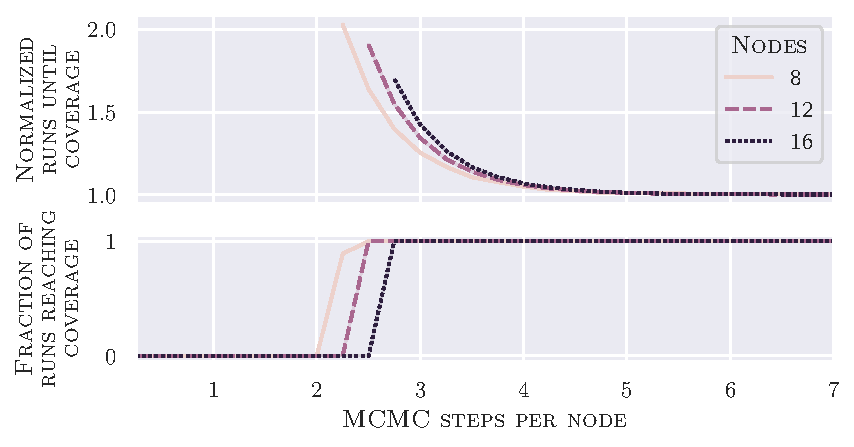
\includegraphics[width=\textwidth]{Figures/experiments/Cov_Cycle.pdf}
    \caption{$C_n$}  
  \end{subfigure}
  \hfill
  \begin{subfigure}{0.325\textwidth}
    \centering
    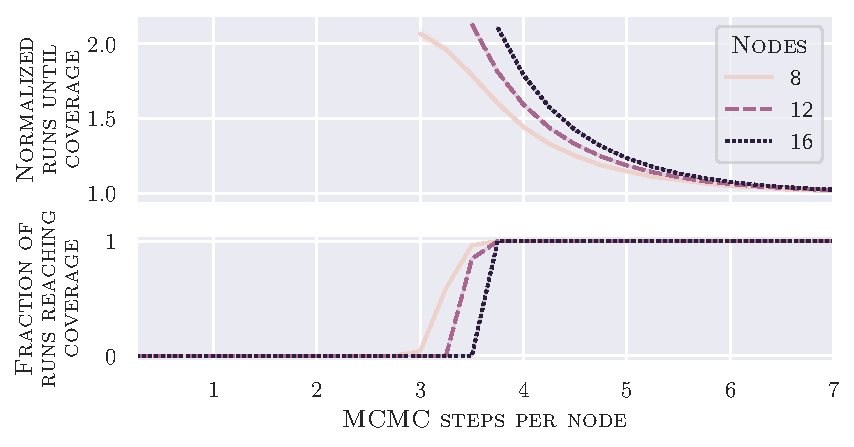
\includegraphics[width=\textwidth]{Figures/experiments/Cov_Nested.pdf}
    \caption{$NC_n$}
  \end{subfigure}
  \hfill
  \begin{subfigure}{0.325\textwidth}
    \centering
    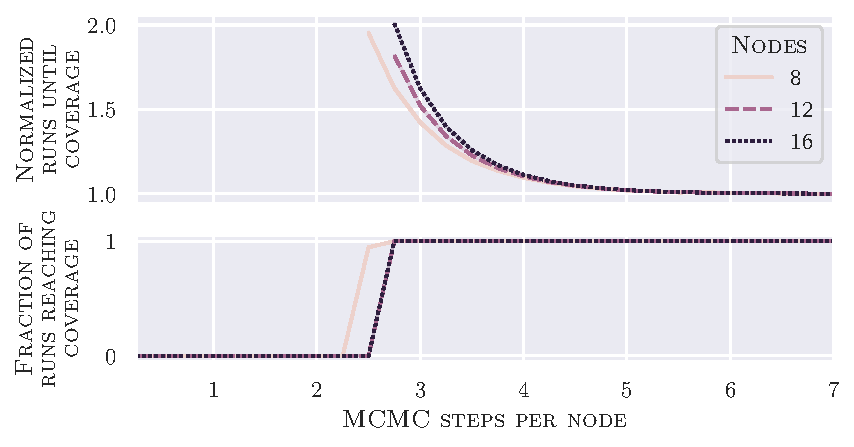
\includegraphics[width=\textwidth]{Figures/experiments/Cov_Paired.pdf}
    \caption{$PC_n$}
  \end{subfigure}
  \caption{
    Runs to see $99\%$ of $\constates$ for $G \in \set{C_n,NC_n,PC_n}$ for $n \in \set{8, 12, 16}$ as function of MCMC steps.
  }
  \label{fig:coverage}
\end{figure}

\cref{fig:coverage} summarizes the results.
As we pick $n$ even, the left cycle of $PC_n$ in fact has one edge less than the right one.

For $C_n$, we find that the exact sampler uses $(4.6 \pm 0.1)|\cstates_{C_n,\wInt}|$ \emph{runs-until-coverage}.
For $NC_n$, the sampler rather uses $(7.0 \pm 0.1)|\cstates_{NC_n,\wInt}|$ and for $PC_n$ $(5.5 \pm 0.1)|\cstates_{PC_n,\wInt}|$ \emph{runs-until-coverage}.
As each sample is a new item with probability of at least $0.01$, this is plausible.

We then replace the exact sampler with the MCMC process for different numbers of steps $\steps$ and measure their \emph{runs-until-coverage}.
This allows us to reject the hypothesis that the MCMC process is identical to the exact sampler if $\steps$ is too small.
If coverage does not occur within $10|\constates|$ steps (\ie more than twice the exact sampler's \emph{runs-until-coverage}), we say that the run does not reach coverage.
We observe a sharp transition from no runs achieving coverage to all runs completing succesfully between $2n \leq \steps \leq 3n$ for $C_n$, between $3n \leq \steps \leq 4n$ for $NC_n$ and again between $2n \leq \steps \leq 3n$ for $PC_n$.
In all cases we see a slight increase in \emph{runs-until-coverage} for bigger $n$ which is consistent with a suplinear mixing time.


\section{Acceptance Rates}\label{sec:exp_acc}
\begin{figure}[!tb]
  \centering
  \makebox[\textwidth][c]{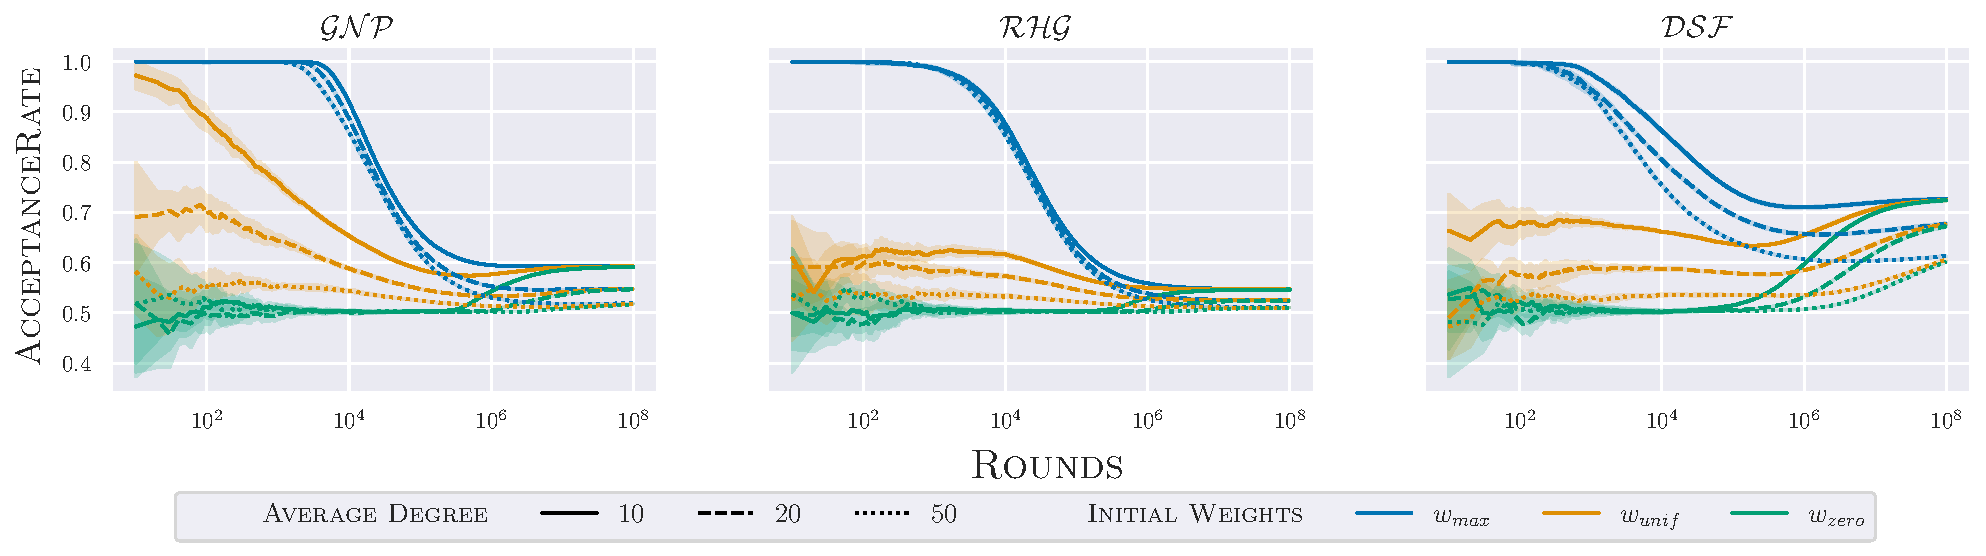
\includegraphics[width=1.2\textwidth]{Figures/experiments/Acc.pdf}}
  \caption{
    Acceptance-Rate over time for different graph models with $n = 10000$ nodes and average degree $\degavg \in \set{10, 20, 50}$
  }
  \label{fig:acc_rates}
\end{figure}

The final measure of \algsl we want to investigate is the the acceptance rate over time, \ie the fraction of rounds in which we accepted the proposed weight change.
This does include weight decreases as well as weight increases.
Therefore, we expect the acceptance rate to converge to some value greater than $0.5$ as we expect weight increases --- which are immediately accepted --- to happen in roughly $50\%$ of the time due to $\wInt$ being symmetric around $0$.
Second, higher number of cycles should result in more rejections and thus a smaller acceptance rate as there are more ways in which a weight decrease could produce a negative cycle.
As higher degrees equate to higher number of cycles, the higher the degree, the lower the acceptance rate.
Lastly, we expect that the higher the average weight of the inital weight function, the higher the acceptance rate in the beginning.
This influence however should diminish over time such that all graphs of the same model with the same number of nodes and edges reach a similar convergence point.

\cref{fig:acc_rates} supports our hypotheses.
Most importantly, all instances of the same model with the same number of nodes and edges converge to the same acceptance rate greater than $0.5$.

Furthermore, regardless of graph model or average degree, instances with an initial weight function $\wmax$ have an acceptance rate of nearly $1.0$ at the beginning before quickly descending between $10^4$ and $10^5$ steps.
Similarly, instances with initial weight function $\wzero$ have an acceptance rate of roughly $0.5$ at the start as roughly every second weight change is a weight increase.
Finally, instances with initial weight function $\wunif$ have starting acceptance rates between those of instances with initial weight functions $\wzero$ and $\wmax$.
Surprisingly, for $\gnp$ graphs with average degree $10$, instances with starting uniform weights also have a nearly $100\%$ acceptance rate at the start.
For $\rhg$ and $\dsf$ graphs, starting acceptance rates for $\wunif$ tend to be centered around $0.6$ (rather $0.5$ - $0.7$).

Additionally, as expected, higher average degrees in fact equate to lower acceptance rates.
This can be seen not only at the final convergence points but also at the beginning and even more exaggerated for $\gnp$ graphs with initial weights $\wunif$. 

Finally, convergence points of $\rhg$ graphs are very close to each other, while the convergence points for $\gnp$ and $\dsf$ graphs are slightly more spread out.
In a similar fashion, $\rhg$ have the smallest convergence points, followed by $\gnp$ and then $\dsf$ graphs.
This could be explained by the fact that in $\rhg$ we have many $2$-cycles which consequently lead to many rejections.
As these $2$-cycles exist regardless of average degree, acceptance rates tend to be closer to each other.
In $\gnp$ graphs, there are longer and fewer cycles which is amplified by a lower average degree whereas in $\dsf$ graphs there are even fewer cycles which leads to even higher acceptance rates.

\bigskip

While all previous measures are no direct proof for a rapid mixing time, they still suggest that the mixing time is bounded by a small polynomial in $m$.
This and the proof in \cref{sec:rapid-mixing} provide compelling evidence for a small mixing time in practice.


\section{Conflict Lengths}\label{sec:exp_conflicts}
The final metrics of the underlying \markov we want to study are \textsc{ConflictLengths} which we introduced in \cref{sec:parallel_sampling}.
Note that accepting rounds in \cref{algo:sampler} however are always global as \algbf does not use pruning and therefore only terminates (accepts) after every node has been visited at least once.
Thus, every weight-decrease that gets eventually accepted generates a round-conflict with at least the most recent accepted weight-decrease.

\begin{figure}[!tb]
  \centering
  \makebox[\textwidth][c]{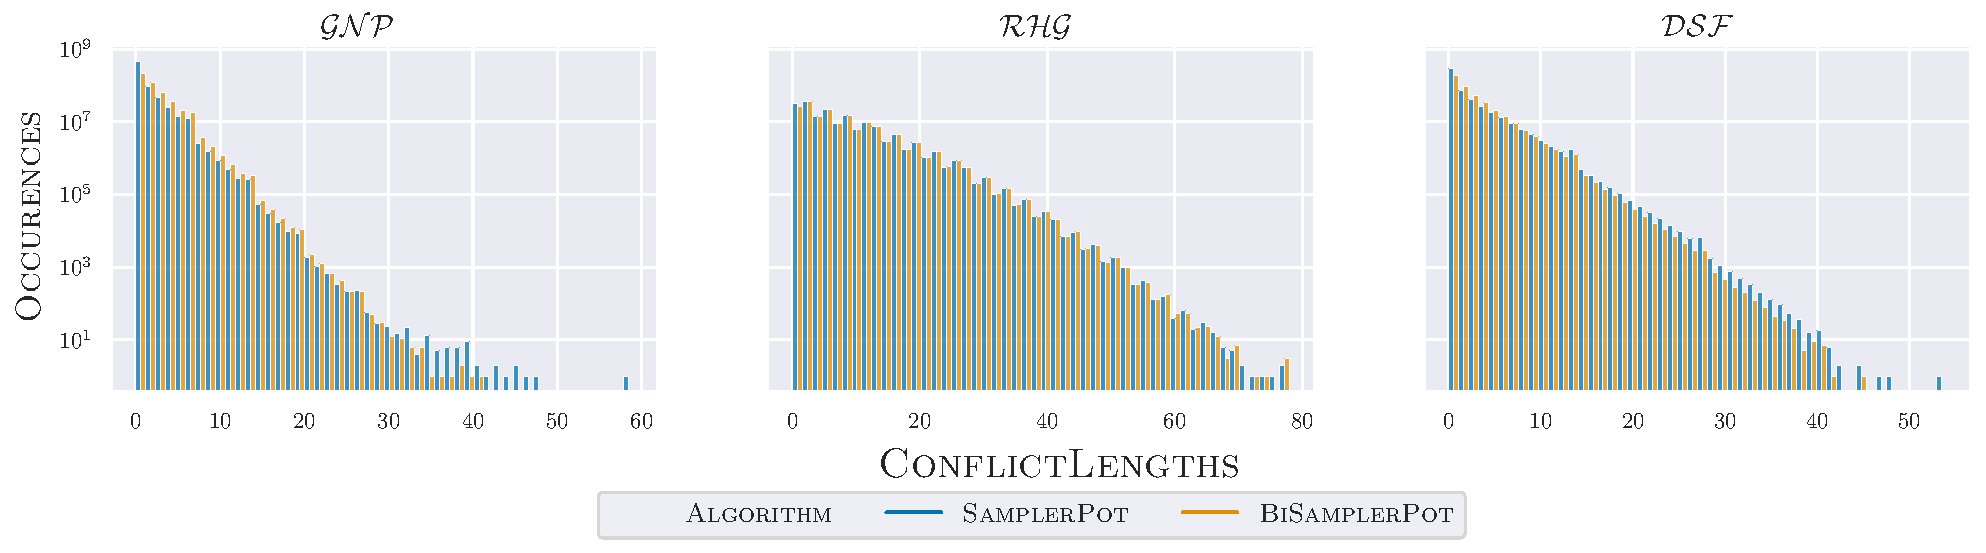
\includegraphics[width=1.2\textwidth]{Figures/experiments/Conflicts_Maximum_10.pdf}}
  \caption{
    Occurences of \textsc{ConflictLengths} between rounds after $10^8$ rounds for different graphs with $n = 10000$ nodes, average degree $\degavg = 10$ and starting weights $\wmax$.
  }
  \label{fig:conflict_lengths_rounds}
\end{figure}

\begin{figure}[!tb]
  \centering
  \makebox[\textwidth][c]{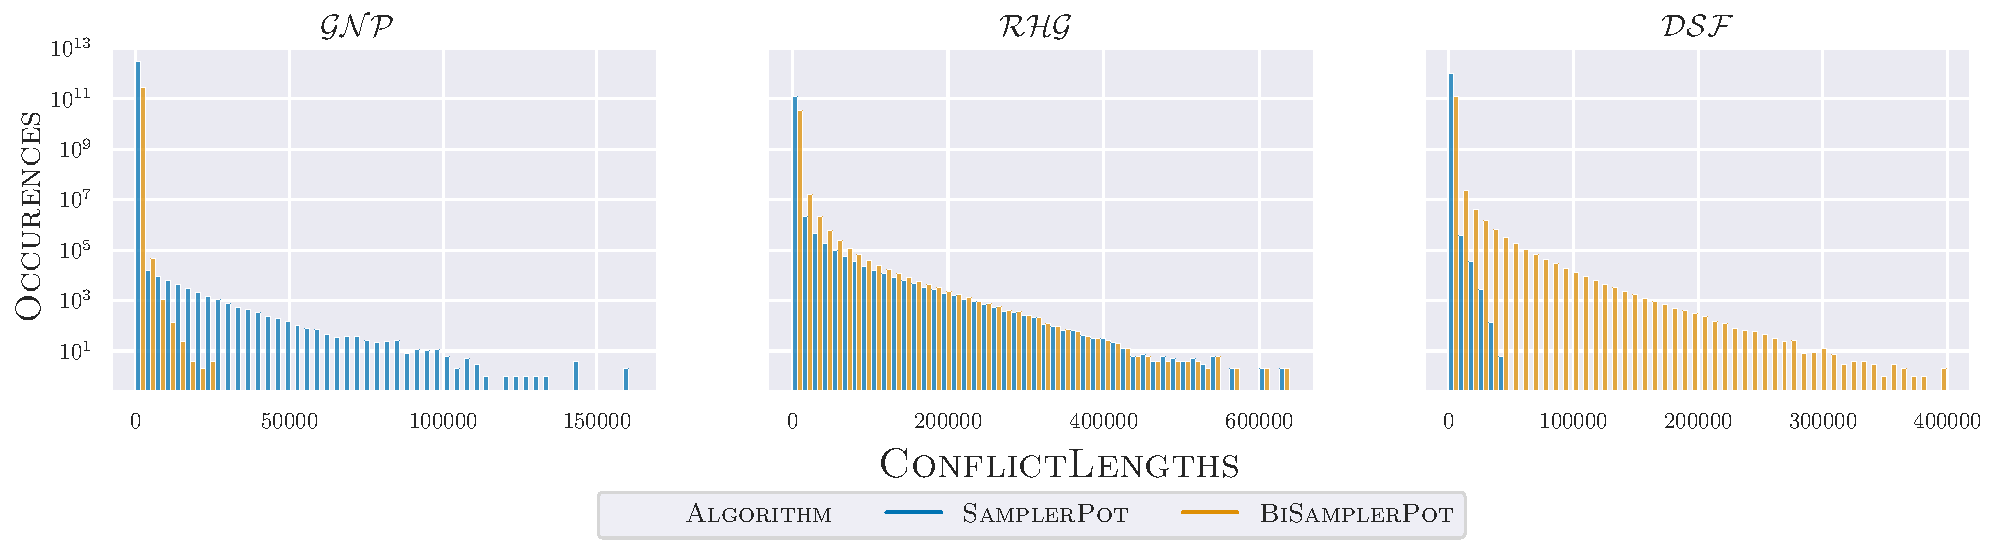
\includegraphics[width=1.2\textwidth]{Figures/experiments/NodeConflicts_Maximum_10.pdf}}
  \caption{
    Occurences of \textsc{ConflictLengths} between nodes after $10^8$ rounds for different graphs with $n = 10000$ nodes, average degree $\degavg = 10$ and starting weights $\wmax$.
  }
  \label{fig:conflict_lengths_nodes}
\end{figure}

Hence, \cref{fig:conflict_lengths_rounds,fig:conflict_lengths_nodes} only depict the distribution of \textsc{ConflictLengths} for \algsp and \algbp for graphs with average degree $10$ and initial weight function $\wmax$.
The complete dataset can be found in the appendix (\cref{fig:app_conflicts_gnp,fig:app_conflicts_rhg,fig:app_conflicts_dsf,fig:app_node_conflicts_gnp,fig:app_node_conflicts_rhg,fig:app_node_conflicts_dsf}).
Although the decline of occurrences for bigger conflict lengths is less steep on \rhg graphs, the general trend is consistent across all different graph classes.
Note that the $y$-axis in the plots is log-scaled while the $x$-axis is not.
Thus, \textsc{ConflictLengths} of rounds seem to follow an almost perfect exponential distribution.
Outliers in all three distributions can be explained by the chosen initial weight function $\wmax$: in early rounds, we almost always can immediately accept a weight change without conducting a thorough search --- a round-conflict basically becomes a node-conflict in these rounds.

While \gnp graphs have one more outlier than \dsf graphs, the distributions are almost identical.
Only \rhg graphs achieve higher average \textsc{ConflictLengths} which is consistent with observations from the previous experiment.
Small cycles and lower acceptance rates lead to siginificantly smaller shortest path trees on average, thus reducing the number of conflicts.

As with all prior metrics, the resulting data is invariant to the initial weight function with the exception of a few outliers.
Also again, a higher average degree leads to more cycles and thus also to lower \textsc{ConflictLengths} on average across all three graph classes.

\medskip

In the case of node-conflicts, the patterns are less consistent.
While, again, the rough trend distributions are invariant to the initial weight function, the impact is way more apparent as for $\wmax$ node-conflicts are incredibly rare in the first $\Oh{m}$ rounds which is more apparent than for round-conflicts (since round-conflicts depend on all nodes). 

The average degrees and graph topology also play a more siginificant role this time.
Surprisingly, for \gnp graphs with average degree $10$, \algsp has far fewer node-conflicts than \algbp --- almost one order of magnitude less.
This however immediately flips for average degrees $20$ and $50$ where \algbp now has far fewer node-conflicts on average than \algsp which can probably be attributed to the fact that partial shortest path trees in \algsp are more likely to have a bigger depth.
Whereas for $\degavg = 10$, most partial shortest path trees are sparse and thus do not include many nodes despite a bigger depth, for larger average degrees this is not the case and a partial shortest path tree with bigger depth includes significantly more nodes leading to more node-conflicts.
For \algbp, which has smaller partial shortest path trees on average and on the extreme, this effect is thus not that apparent.

The same steep decline of \algsp for higher average degrees can also be observed for \rhg graphs.
Although, \algbp performs equally good for average degree $10$ in that case.
Finally, for \dsf graphs, \algbp has far fewer node-conflicts in all cases, regardless of average degree and weight function.

Notice however that this decline also happens for \algbp.
Higher average degrees and thus more edges lead to smaller \textsc{ConflictLengths} for both algorithms in \gnp and \rhg graphs.
This decrease however has an higher impact on \algsp compared to \algbp which again is consistent with prior observations.
Also, due to the very small cycles in \rhg graphs, the choice of algorithm does make a big impact for low average degrees.

Finally, the most surprising observation is the fact that \textsc{ConflictLengths} seem to increase for higher average degrees in \dsf graphs.
One possible explanation points again back at acceptance rates where \dsf graphs had by far the biggest decrease in acceptance rate for higher average degrees (more than $12\%$ from $\degavg = 10$ to $\degavg = 50$).
This, coupled with the already very acyclic nature of \dsf graphs could then lead to very short rejecting paths which incur less node-conflicts overall.

\bigskip

Nonetheless, a more detailed investigation of \textsc{ConflictLengths} seems warranted to better understand the behaviour of the underlying \markov as well as the distributions of shortest paths in such random graphs. 



\section{Sequential Algorithms}\label{sec:exp_seq}
In this section, we want to study performance metrics of the various sequential algorithms proposed in \cref{sec:uniform_sampling}, namely \algsl, \algsp, and \algbp.
For each parameter setting, we run all three algorithms simultaneously in each round (back to back) to obtain the desired performance metrics on the same dataset for a fair comparison.\footnote{
  This also served as an additional correctness check for these algorithms as we could assert equality of their output (\emph{accepted} or \emph{rejected}) in each round. 
}

As \algsl uses \algbf as a subroutine which is inherently slow, it is not feasible to run all $10^8$ rounds of the MCMC in each instance for \algsl.
Instead, we opt for an amortized approach and only ran \algbf every $10^3$ rounds for $\steps > 10^6$.
For $\steps \leq 10^6$, we run \algbf every $\max\left\{1,10^{\ceil{\log_{10}(\steps)} - 4}\right\}$ rounds, \ie for $10^i < \steps \leq 10^{i + 1}$, we obtain $\min\left\{10^4 - 10^3,10^{i + 1} - 10^i\right\}$ datapoints of \algbf.
Metrics such as runtime are then averaged out.
Further discussed in \cref{sec:exp_time}, this has no significant impact on the obtained data and is coherent with test runs that executed \algbf every round.

\subsection{Queue Insertions}
\begin{figure}[!tb]
  \centering
  \makebox[\textwidth][c]{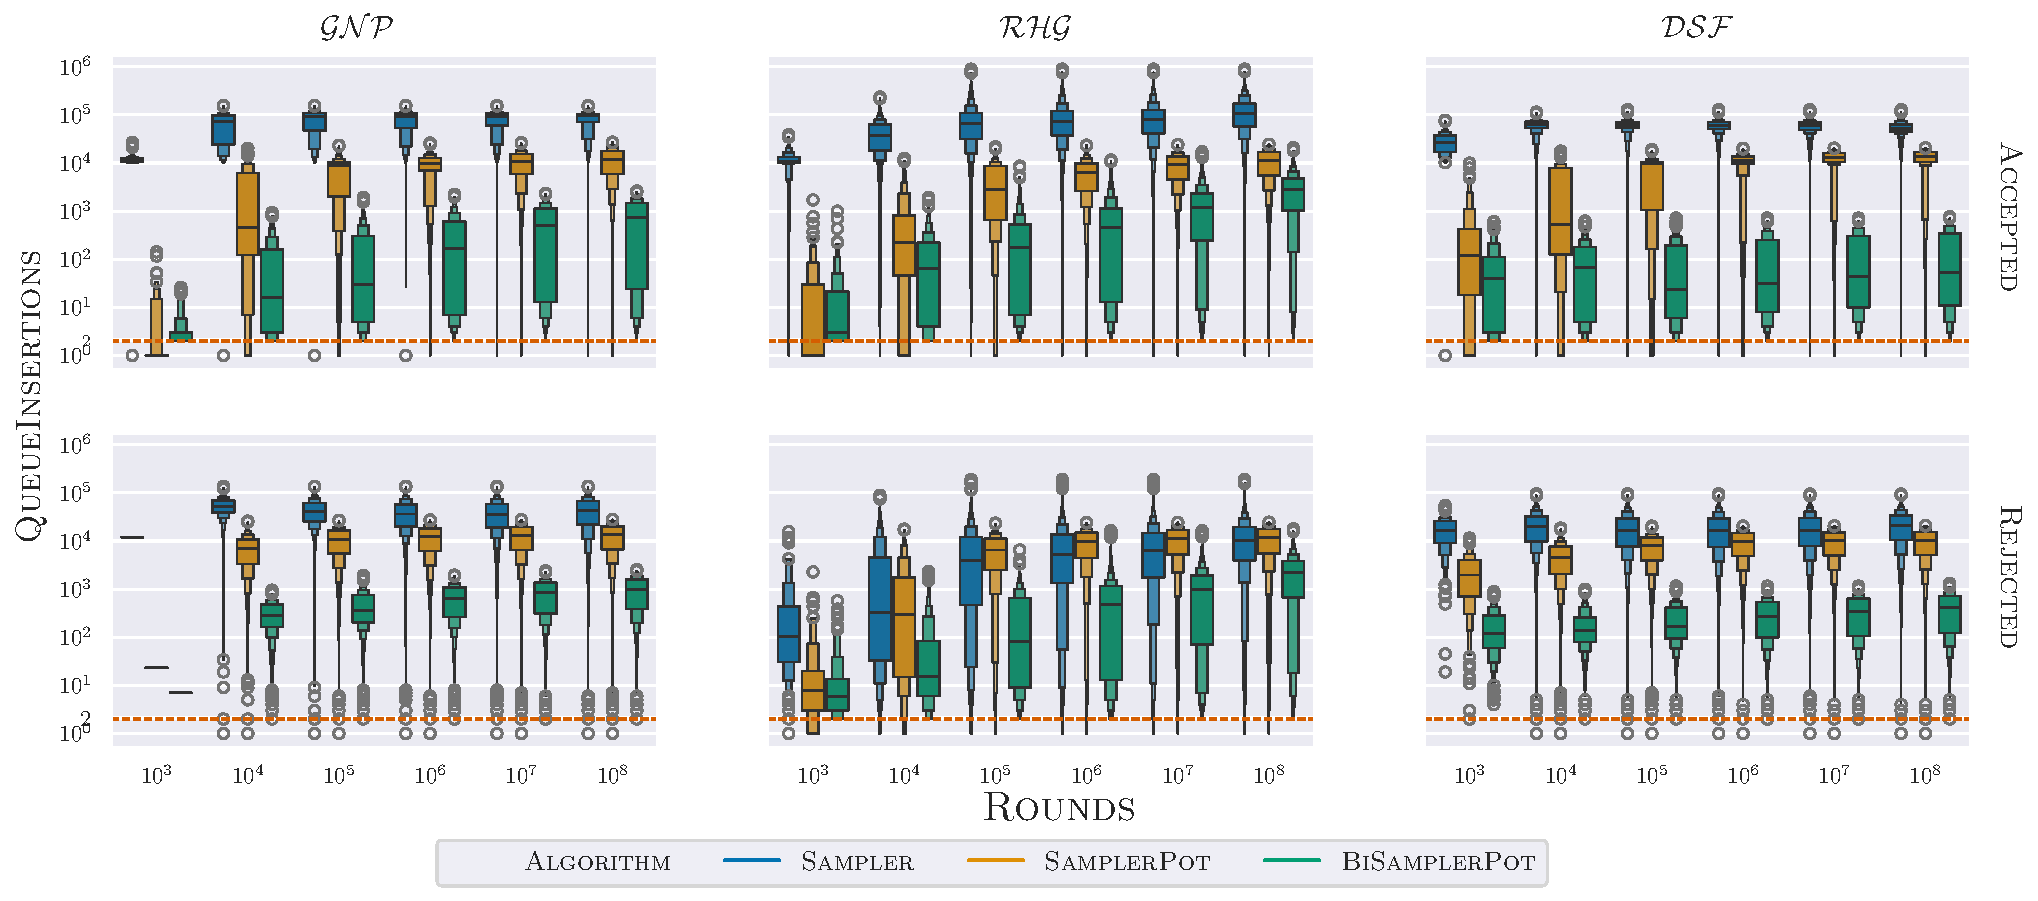
\includegraphics[width=1.2\textwidth]{Figures/experiments/Ins_Max_10.pdf}}
  \caption{
    Number of Queue-Insertions per algorithm for different graphs with $n = 10000$ nodes and average degree $\degavg = 10$ with starting weights $\wmax$.
  }
  \label{fig:ins}
\end{figure}

The first metric we want to investigate is the number of queue insertions of the underlying shortest path queries (\algbf, \algdk, \algbd).
For \algbf, this is the number of queue insertions in the SPFA heuristic, for \algdk and \algbd the number of priority queue insertions.
We further differentiate between \emph{accepted} and \emph{rejected} rounds.

It is a common observation that in practice, worst-case bounds of \algbf tend to be overly pessimistic.
Additionally, as mentioned before, bidirectional searches perform significantly better than their unidirectional variants.
This is supported by \cref{fig:ins} where we can see the distribution of Queue-Insertions over time for \algbf, \algsp, and \algbp for graphs with average degree $10$ and initial weights $\wmax$.
Again, the complete dataset is found in the appendix (\cref{fig:app_ins_gnp,fig:app_ins_rhg,fig:app_ins_dsf}).

\algbf is by far the worst algorithm among all three.
As \algdk and \algbd can also significantly prune their search space, this is even more apparent for \emph{accepted} rounds where a \algbf iteration only ends after the complete shortest path tree was discovered whereas \algdk and \algbd can stop after computing partial shortest path trees.
Surprisingly, in \emph{accepted} rounds, \algdk performs in the median better than \algbd, although this can be attributed to super short rounds with only $1$ insertion (the starting one).
While \algdk only terminates when its queue is empty, \algbd terminates when \emph{rejecting} path is disproven - often with leftover elements in its queue.
Nonetheless, as we will see later in \cref{fig:ins_per_wu}, the average number of Queue-Insertions is much smaller for \algbd as it is for \algdk overall.

For \emph{rejected} rounds however, the order of medians is flipped and \algbd performs significantly better than \algdk; whereas in \emph{accepted} rounds, both \algdk and \algbd performed on average less than
$10$ insertions, in \emph{rejected} rounds, \algbd is a whole order of magnitude better ($10^2\sim 10^3$ compared to $10^3\sim 10^4$).
Still, \algbf performs the worst, although the difference to \algdk is not that apparent as before anymore: instead of multiple orders of magnitude, \algbf is at most $10$ times worse than \algdk.
This is coherent with theory as both \algbf and \algdk need to find the same path that leads to \emph{rejection}: pruning no longer allows for early returns.


\subsection{Potential Updates}
\begin{figure}[!tb]
  \centering
  \makebox[\textwidth][c]{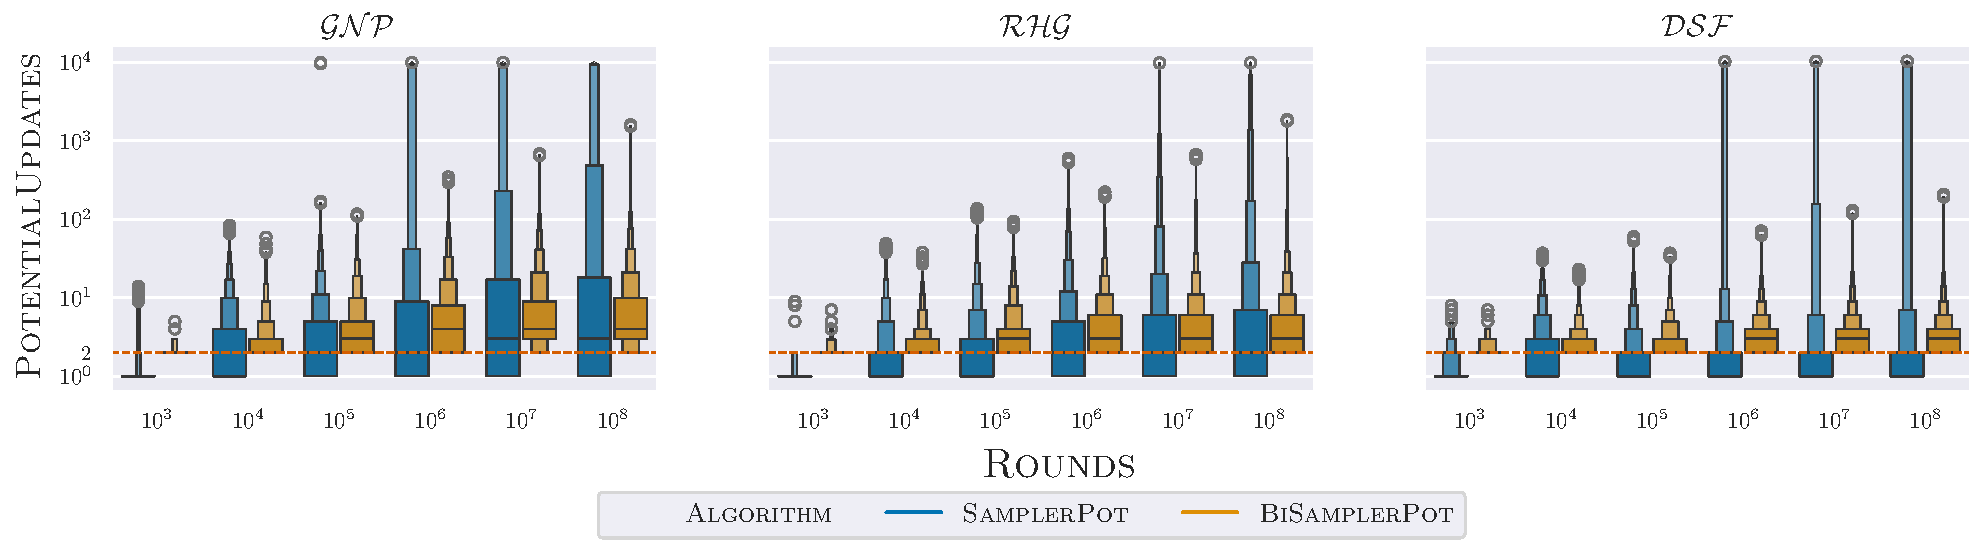
\includegraphics[width=1.2\textwidth]{Figures/experiments/Pot_Max_10.pdf}}
  \caption{
    Number of Potential-Updates per algorithm for different graphs with $n = 10000$ nodes and average degree $\degavg = 10$ with starting weights $\wmax$.
  }
  \label{fig:pot}
\end{figure}

A similar point of comparison is the number of potential updates incurred by an \emph{accepted} weight change.
As \algbf does not rely on potentials, this only applies to \algdk and \algbd in \emph{accepted} rounds.
\cref{fig:pot} show similar trends observed in \cref{fig:ins}.\footnote{
  The complete data can be seen in \cref{fig:app_pot_gnp,fig:app_pot_rhg,fig:app_pot_dsf}.
}

While \algdk seems to perform better in the median, on average, \algbd still outperforms \algdk as it has far fewer and smaller extremes.
For example, ignoring all datapoints of $\leq 2$ potential updates actually leads to a smaller median for \algbd.

The occurences of extremes are further amplified by higher average degrees as a potential change can incur significantly more cascading potential changes.
The choice of an initial weight function also impacts the number of potential updates as for \wmax, both algorithms had a significant number of direct \emph{accepts} ($1$ or $2$ potential updates) in the first $10^5$ rounds: if that is not the case, \ie for \wunif, the median and subsequently the average rises for both algorithms, although only at the beginning.
At the end, the number of potential updates seems to be again independent of initial weight function.
Note that for $\wzero$ there are almost no potential changes in the first $10^6$ rounds as almost all accepted weight changes are weight increases while almost all weight decreases are rejected.\footnote{
  Remember that in our setting, we have at least $10^5$ edges and we expect to have seen every edge with high probability after $m \cdot \log(m) > 10m \geq 10^6$ steps. 
}


\subsection{Average Runtime}\label{sec:exp_time}
\begin{figure}[!tb]
  \centering
  \makebox[\textwidth][c]{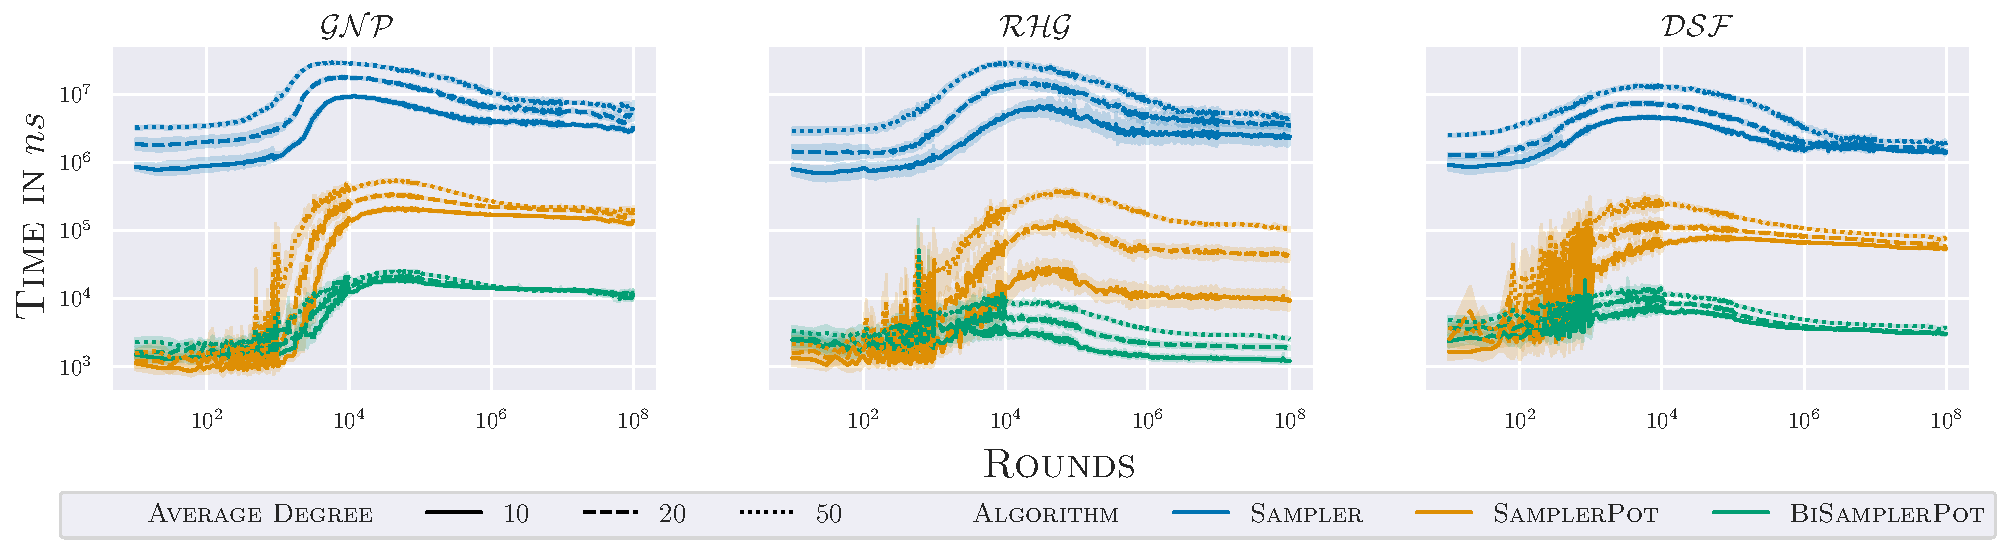
\includegraphics[width=1.2\textwidth]{Figures/experiments/Time_Maximum.pdf}}
  \caption{
    Runtime per round over time of different algorithms for different graph models with $n = 10000$ nodes and average degree $\degavg \in \set{10, 20, 50}$ with initial weight function $\wmax$.
  }
  \label{fig:time}
\end{figure}

Lastly, we study the performance of our implementations through a time measurement.
\cref{fig:time} shows the average runtime per round over time for all three algorithms and different average degrees.\footnote{
  \cref{fig:app_time} shows the data for all initial weight functions.
}

They further emphasize earlier observations for Queue-Insertions and Potential-Updates.
\algbd is by far the best algorithm: being roughly $10$ times faster on average than \algdk and $100\sim1000$ faster than \algbf.
Furthermore, \algdk is also $10\sim100$ times faster than \algbf confirming our expectations.

Also, runtime appears to increase with higher average degrees as more edges are present and thus traversed in the algorithms.
Following the previous observations on Queue-Insertions, instances that start with \wzero are faster at the beginning for \algbf as \emph{rejecting} rounds are computationally faster due to early returns.
Surprisingly, algorithms seem to perform better on average on \rhg graphs compared to \gnp and \dsf graphs: probably due to shorter cycles.

The measurements are very noisy at the beginning --- probably due to very short rounds on average that lead to many inconsistencies in the very few instances that we run.
However, with time, they even out as the \markov settles into a stable state.

Finally, the initial weight function again has no siginificant impact on the runtime of the algorithms.


\section{Batching}\label{sec:exp_batch}
We give a short overview over the performance of \algbt with $64$ threads compared to \algbp.
\cref{tab:par_batching_perf} summarizes all total runtimes on all possible input parameters.

\begin{table}[!tb]
    \begin{center}
        \begin{tabular}{c|c|c|c|c|c}
            \multirow{2}{*}{Graph} & \multirow{2}{*}{\shortstack{Average \\ Degree}} & \multirow{2}{*}{\shortstack{Initial \\ Weights}} & \multirow{2}{*}{\shortstack{\algbp \\ time in $ms$}} & \multirow{2}{*}{\shortstack{\algbt \\ time in $ms$}} & \multirow{2}{*}{\shortstack{Average \\ Slowdown}} \\ & & & & & \\ \hline
           $\mathcal{DSF}$ & $10$ & \textsc{Maximum} & $10414 \sim 11257$ & $1796183 \sim 1925397$ & $172.43$ \\
            &  & \textsc{Uniform} & $10752 \sim 11385$ & $1821850 \sim 1958901$ & $169.408$ \\
            &  & \textsc{Zero} & $10684 \sim 11191$ & $1850585 \sim 1956106$ & $174.093$ \\
            & $20$ & \textsc{Maximum} & $12712 \sim 13314$ & $2026321 \sim 2174308$ & $160.966$ \\
            &  & \textsc{Uniform} & $13494 \sim 14126$ & $2119665 \sim 2241692$ & $157.143$ \\
            &  & \textsc{Zero} & $13389 \sim 13780$ & $2142839 \sim 2247288$ & $161.368$ \\
            & $50$ & \textsc{Maximum} & $19154 \sim 20743$ & $2332546 \sim 2456868$ & $121.462$ \\
            &  & \textsc{Uniform} & $20246 \sim 21162$ & $2445529 \sim 2568598$ & $121.048$ \\
            &  & \textsc{Zero} & $19558 \sim 20160$ & $2449341 \sim 2564978$ & $125.72$ \\
           $\mathcal{GNP}$ & $10$ & \textsc{Maximum} & $33441 \sim 35232$ & $2187103 \sim 2322490$ & $65.001$ \\
            &  & \textsc{Uniform} & $34187 \sim 35661$ & $2199807 \sim 2316110$ & $64.215$ \\
            &  & \textsc{Zero} & $33137 \sim 34544$ & $2182611 \sim 2315062$ & $65.882$ \\
            & $20$ & \textsc{Maximum} & $33721 \sim 34966$ & $2344612 \sim 2484474$ & $69.878$ \\
            &  & \textsc{Uniform} & $34453 \sim 35873$ & $2383430 \sim 2482532$ & $68.833$ \\
            &  & \textsc{Zero} & $33026 \sim 34098$ & $2343049 \sim 2480880$ & $71.109$ \\
            & $50$ & \textsc{Maximum} & $33689 \sim 36420$ & $2503518 \sim 2650046$ & $73.677$ \\
            &  & \textsc{Uniform} & $34396 \sim 36178$ & $2496346 \sim 2614062$ & $72.805$ \\
            &  & \textsc{Zero} & $29944 \sim 31783$ & $2333914 \sim 2514262$ & $79.856$ \\
           $\mathcal{RHG}$ & $10$ & \textsc{Maximum} & $3300 \sim 5704$ & $474456 \sim 1592833$ & $181.366$ \\
            &  & \textsc{Uniform} & $3167 \sim 10026$ & $496726 \sim 1199446$ & $175.603$ \\
            &  & \textsc{Zero} & $3219 \sim 7115$ & $432652 \sim 1345578$ & $176.604$ \\
            & $20$ & \textsc{Maximum} & $4587 \sim 12695$ & $717543 \sim 1324089$ & $171.328$ \\
            &  & \textsc{Uniform} & $4738 \sim 7312$ & $689240 \sim 1619917$ & $190.424$ \\
            &  & \textsc{Zero} & $4407 \sim 18096$ & $697825 \sim 1677583$ & $185.791$ \\
            & $50$ & \textsc{Maximum} & $7698 \sim 13562$ & $1114689 \sim 1872249$ & $143.872$ \\
            &  & \textsc{Uniform} & $7574 \sim 13659$ & $1069077 \sim 1864137$ & $146.277$ \\
            &  & \textsc{Zero} & $6721 \sim 16275$ & $971226 \sim 1959928$ & $148.194$ \\
        \end{tabular}
    \end{center}

    \caption{Runtime of \algbp and \algbt ($64$ Threads) with $10^8$ rounds for different graphs with $10^4$ nodes.}
    \label{tab:par_batching_perf}
\end{table}

Consistent with the results on round-conflicts, regardless of chosen graph or weight function, \algbt is multiple times ($64\sim190$) slower than \algbp due to the sheer amount of additional work and overhead.
On \rhg and \dsf graphs, the slowdown is twice as bad as on \gnp graphs which indicate that \qq{scale-free} graphs are harder to handle for \algbt.
While our implementation is not highly optimized and one could probably make the algorithm a bit faster, the sheer difference in performance as well as the theoretical limit imposed by round-conflicts pose significant challenges for \algbt to ever reach \algbp's performance in practice.
The additional overhead of parallelization can only then be counteracted if another way of resolving conflicts is found.
In the current state, this is not a feasible solution.



\section{Neighborhood Updates}\label{sec:exp_neighbor}
In our final experiments, we want to compare \algbp (and \algsp) to \algns.
While \algns is no true parallel algorithm as it is again sequential in its core, it \qq{parallelizes} weight-updates by performing multiple in one round.
Thus, as our goal in the \markov is to permute the weights as much as possible to get a coherent sample of the target distribution, we measure the performance of \algns with regard to succesfull weight-updates.
Note that since \algns is siginificantly slower per round than \algbp or \algsp as we perform multiple updates instead of one, we only ran \algns for $10^7$ rounds compared to $10^8$ for \algbp and \algsp.

\subsection{Queue Insertions per Weight Change}
We first compare Queue-Insertions per weight-update for all three algorithms.

\begin{figure}[!tb]
  \centering
  \makebox[\textwidth][c]{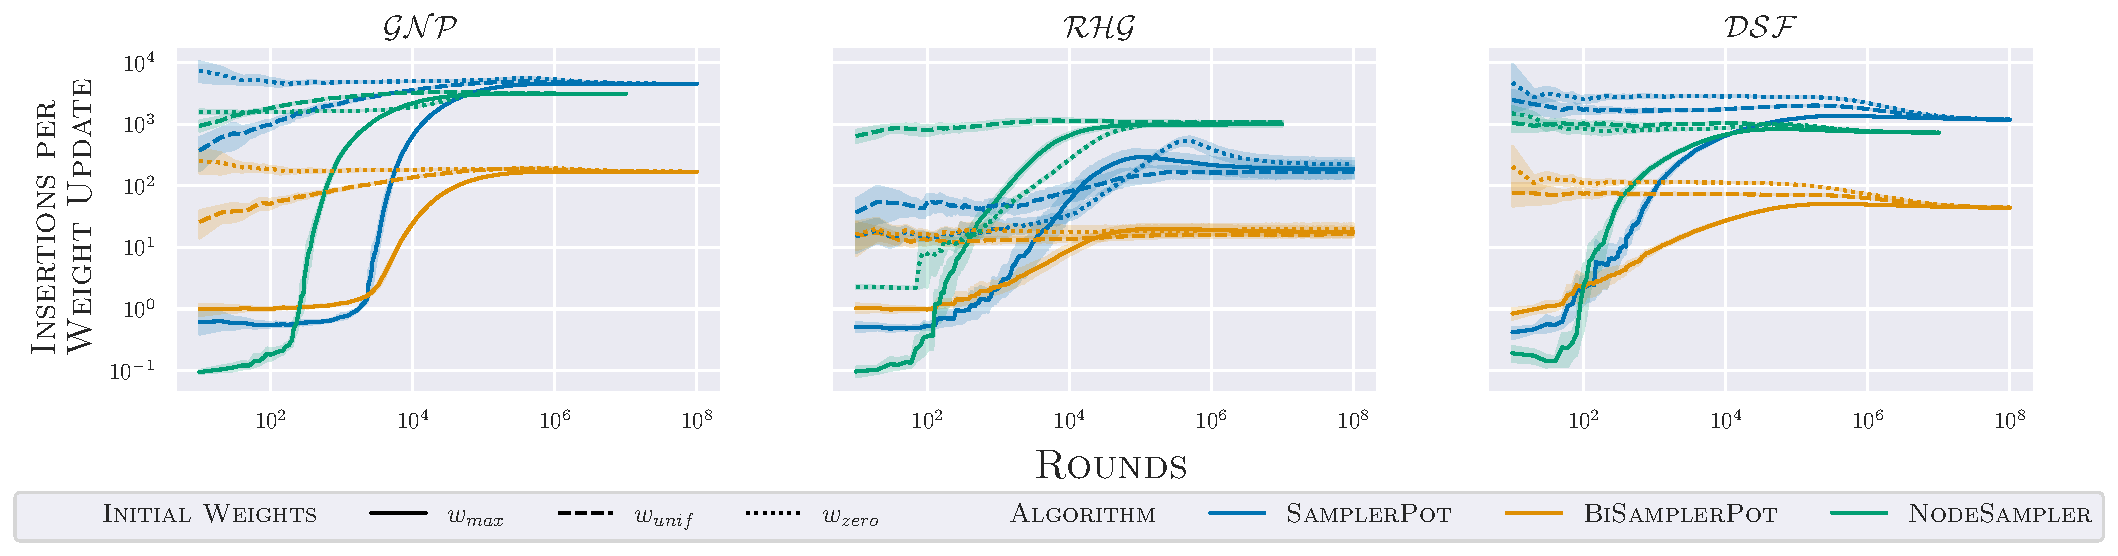
\includegraphics[width=1.2\textwidth]{Figures/experiments/InsPerWU_10.pdf}}
  \caption{
    Number of Queue-Insertions per succesfull Weight-Update over time of different algorithms on different graphs with $n = 10000$ nodes and average degree $\degavg = 10$ for starting weights $w_{init} \in \set{\wmax, \wunif, \wzero}$.
  }
  \label{fig:ins_per_wu}
\end{figure}

See \cref{fig:ins_per_wu} for the results on graphs with average degree $10$.
The complete dataset can be seen in \cref{fig:app_ins_per_wu}.
As one would expect, the initial weight function again has no significant impact.

Since \algsp and \algbp operate on the same underlying \markov, the number of succesfull weight updates is similar\footnote{
  In our case, it is even equal as our experiment for \algbf, \algsp, and \algbp (where this data was obtained from) ran on one graph at a time, meaning acceptance of weight-updates was invariant to the sampling algorithm.
} and the relation between \algbp and \algsp remains similar to those in the previous Queue-Insertion experiment.
Although, we now get more insight into the average number of Queue-Insertions as compared to distributions as a whole.
Therefore, it is even more apparent that \algbp is far better than \algsp.

Surprisingly, while \algbp is also far better than \algns regardless of graph class, \algns is slightly better for \gnp and \dsf graphs whereas for \rhg graphs, \algsp slightly has the edge.
Nonetheless, \algbp is almost always at least one order of magnitude better than both \algsp and \algns.

This observation also extends to higher average degrees where \algbp still is by far the best algorithm.
Only for \dsf graphs with an average degree of $50$, \algns gets reasonably close to \algbp (although still worse).

For \gnp and \rhg graphs, the order of \algsp and \algns is flipped only for average degree $20$.
Similarly, while \algns is better on \dsf graphs than \algsp, for average degree $20$ this difference is the smallest among all three (average degrees).
This can probably be attributed to the fact that for very small average degrees, the shortest path trees of \algns are not much bigger than those of \algsp because the graphs are very sparse.
Nonetheless, \algns performs more weight-updates for a single shortest path tree on average.
This is no longer true for higher average degrees ($20$) as now the shortest path trees get bigger which is more noticeable in \algns where the pruning parameter is bigger on average.
For even bigger average degrees ($50$) however, the number of incoming edges of a node and thus also the number of edges for which a weight-change is proposed is significantly higher again.
At this point, the number of succesfull weight-updates grew faster than the size of the computed shortest path trees, hence \algns now performing better than \algsp again.



\subsection{Potential Updates per Weight Change}
This follow up experiment studies the number of potential updates per succesfull weight-update.

\begin{figure}[!tb]
  \centering
  \makebox[\textwidth][c]{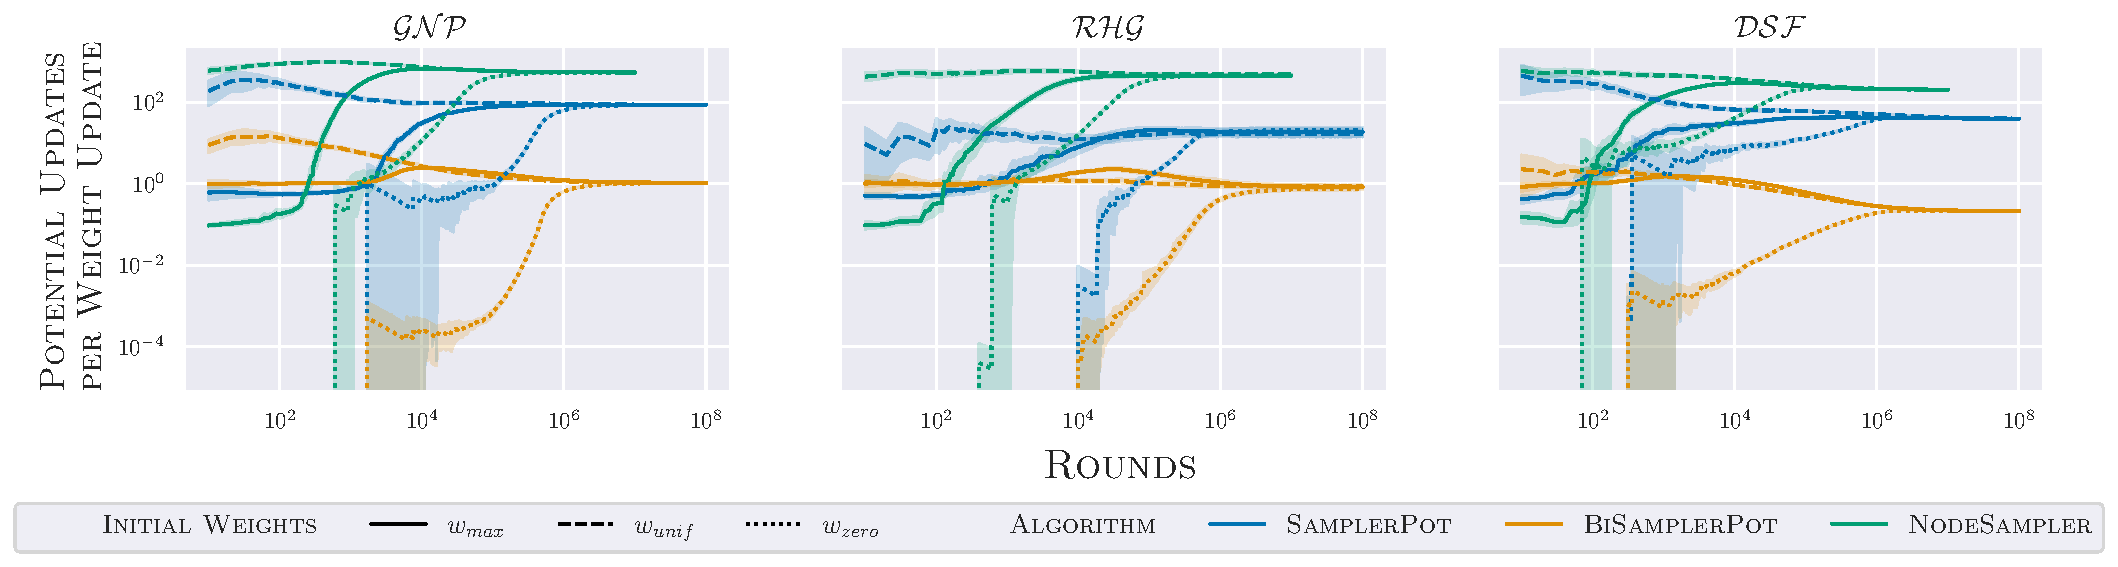
\includegraphics[width=1.2\textwidth]{Figures/experiments/PotPerWU_10.pdf}}
  \caption{
    Number of Potential-Updates per succesfull Weight-Update over time of different algorithms on different graphs with $n = 10000$ nodes and average degree $\degavg = 10$ for starting weights $w_{init} \in \set{\wmax, \wunif, \wzero}$.
  }
  \label{fig:pot_per_wu}
\end{figure}

\cref{fig:pot_per_wu} again depicts the results for graphs with average degree $10$.
See \cref{fig:app_pot_per_wu} for the complete data.
Note that since $\wzero$ has almost no succesfull weight-decreases at the beginning due to the already very low weight, potential updates only happen after roughly $10^3$ rounds.

Again, similar trends as for Queue-Insertions per succesfull weight-update can be observed.
The only very apparent difference is that now \algsp performs far better than \algns across all categories.
Since, potential updates are only performed in accepted rounds in \algsp, the number of Queue-Insertions in \algsp is inflated with rounds where no potential-update was performed afterwards.
In comparison, in \algns, we almost always accept at least one weight change which in turn incurs potential-updates.

Nonetheless, \algbp is again by far the best algorithm among all three.

\subsection{Runtime per Weight Change}
The final experiment compares the average runtime per succesfull weight-update (see \cref{fig:time_per_wu,fig:app_time_per_wu}). 

\begin{figure}[!tb]
  \centering
  \makebox[\textwidth][c]{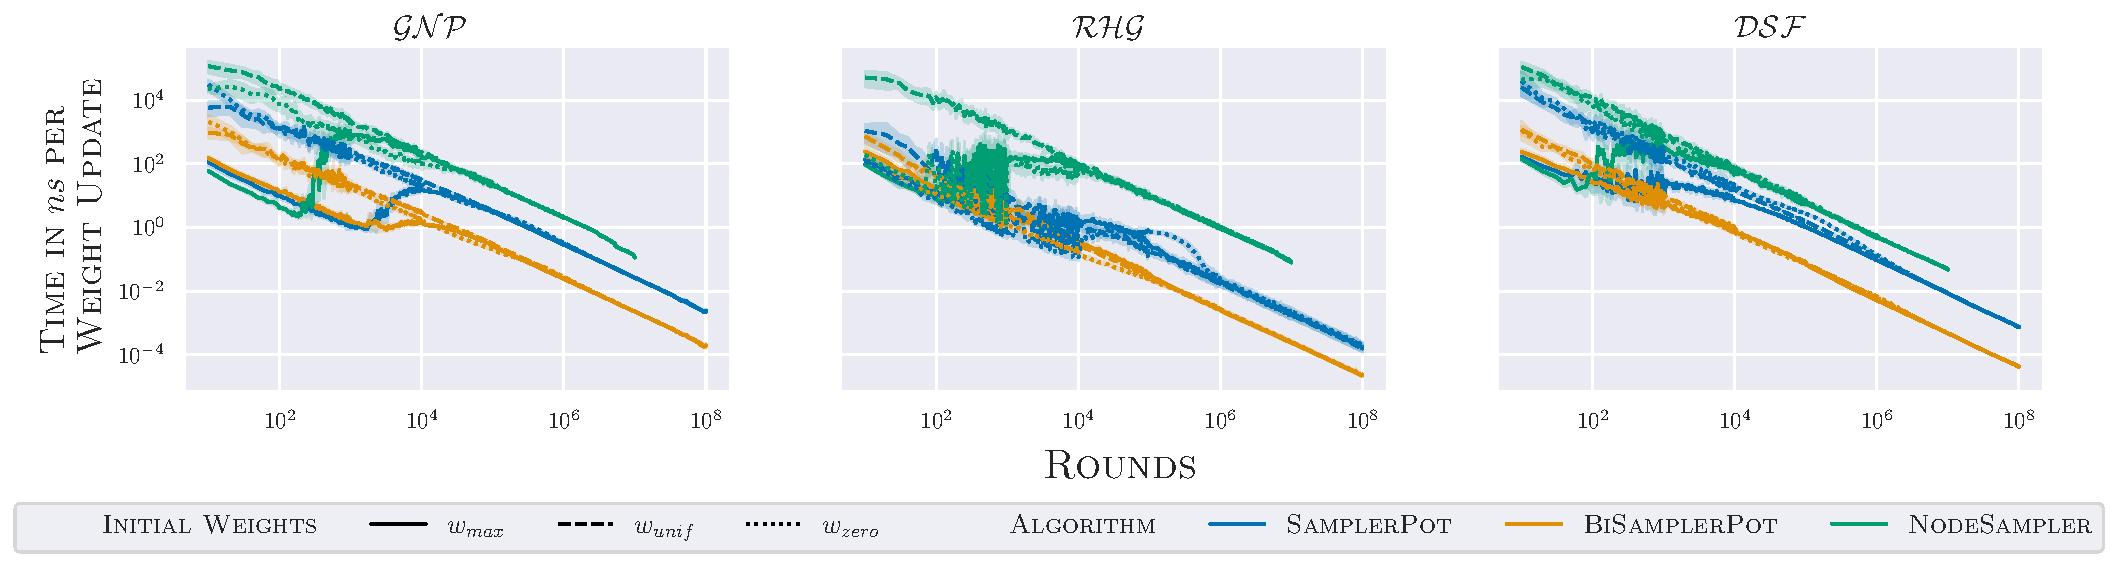
\includegraphics[width=1.2\textwidth]{Figures/experiments/TimePerWU_10.pdf}}
  \caption{
    Runtime per succesfull Weight-Update over time of different algorithms on different graphs with $n = 10000$ nodes and average degree $\degavg = 10$ for starting weights $w_{init} \in \set{\wmax, \wunif, \wzero}$.
  }
  \label{fig:time_per_wu}
\end{figure}

The results are basically an extension of the previous experiment: \algbp is again the fastest algorithm, followed by \algsp and finally \algns --- regardless of average degree or initial weight function.
The only upset to this happens in \dsf graphs where \algns appears to be slightly faster at the end than \algsp which could warrant further experiments.
However, since \algsp fares much better in the first $10^6$ rounds, this speedup probably does not matter much in practice since \algsp is significantly faster in the beginning.
Furthermore, \algbp should still always be the preferred sampling algorithm.



